\documentclass{article}
\usepackage{graphicx}
\usepackage[a4paper, total={7in, 9in}]{geometry}
\usepackage[Algorithm]{algorithm}
\usepackage[noend]{algpseudocode}
\usepackage{amsmath}
\usepackage[italian]{babel}
\usepackage{stmaryrd}


 \MakeRobust{\Call}

\title{ \textbf{ Kernel Image Proccesing} }
\author{ \textbf{ Elmir Šut} \\ \href \\ \href UP FAMNIT \\ \href{E-mail:\textit{elmirsutisz@gmail.com} }}
 
 \makeatletter
\setlength{\@fptop}{0pt}
\setlength{\@fpbot}{0pt plus 1fil}
\makeatother

\begin{document}
\twocolumn
\date{25.12.2019}
\maketitle

\begin{textit}

{This report will present a framework for calculating convolution of each pixel in an image using convolution matrix(kernel). In particular, the main focus was on using edge detection convolution matrices when solving calculations sequentially, in parallel using multiple threads and with
message passing between multiple single-threaded processes (MPI). Measurements were recorded and played key role in deciding our final solution. 

Using simple GUI (graphical user interface) results will be shown interactively with a final image and time taken to process it using  the aforementioned programs.}
 
\end{textit}

\section{Introduction}

The smallest segment of an image is a pixel, depicted as square. Every single image is two-dimensional graphics determined by width and height, measured in pixels. Each pixel has strictly determined place and it is defined by number of bits used to save it in memory.  

Pixels in monochrome images  consist of one value which represents light intensity or specific shade of grey, but in color images three values (Red, Green and Blue) are needed to create one pixel. Therefore color image is consisted of three same-size matrices, each representing one color among aforementioned color channels.

Convolution is a process  where we add value of each pixel weighted by convolution matrix to its local neighbours where as a result we get new value for current pixel.\\
\\
The general expression of a convolution is: 


 $
{\displaystyle g(x,y)=\omega *f(x,y)=\sum _{s=-a}^{a}{\sum _{t=-b}^{b}{\omega (s,t)f(x-s,y-t)}}} 
 $
 
 
where  \textit{g(x,y)}  is the convoluted image, \textit{f(x,y)}  \justify is the image to be convoluted, $ \omega $ is the convolution matrix. Every element of the convolution matrix is considered by $  {\displaystyle -a\leq s\leq a}{\displaystyle -a\leq s\leq a} $ and ${\displaystyle -b\leq t\leq b}{\displaystyle -b\leq t\leq b}.$ \footnote{WIKIPEDIA: https://bit.ly/2EKU1dh}\\

\begin{algorithm}[tbph]
\caption{Sequential Convolution }
\label{alg:MYALG}
\begin{algorithmic}[1]
\Function{convolute(input, width, height, kernel, kernelW, kernelH)}{}
\State $\textit{smallWidth} \gets \text{width - kernelWidth + 1}\textit{}$
\State $\textit{smallHeight} \gets \text{height - kernelHeight+ 1}\textit{}$
\State $\textit{output} \gets \text{height$  {\bigtimes}{\vartimes} $width}\textit{}$ 

\For {$i \gets 0$ to $smallWidth$}
 \State \For {$j \gets 0$ to $smallHeight$}
   \State $output(i+1,j+1)\gets \textit{SPC(input, i, j, kernel, kernelWidth, kernelHeight)}$\\
   \EndFor $\textbf{end for}$\\
 \State \EndFor $\textbf{ end for}$\\
 \State $\textbf{ return } output$
 
\endFunction\\

\Function{spc(input, x, y, kernel, kernelW, kernelH)}{}
\State $\textit{accumulator} \gets \text{0}\textit{}$
\For {$i \gets 0$ to $kernelWi$}
 \State \For {$j \gets 0$ to $kernelH$}
   \State $accumulator\gets \textit{accumulator} + input(x+i,y+j) * kernel(i,j)$\\
   \EndFor $\textbf{end for}$\\
 \EndFor $\textbf{ end for}$
 \State $\textbf{ return } accumulator$
\\
\\


\Comment{ Total complexity of this algorithm will be defined by smallWidth, smallHeight, kernelW and kernelH so we can represent it as: 
 \displaystyle O(smallWidth*smallHeight* kernelW* kernelH )}

\Comment{Considering special case when image is square-shaped$\displaystyle (width == height), $ and  kernel is square-shaped$\displaystyle (kernelW == kernelH), $ then our complexity would be  \displaystyle O((N*M)^2)}

\end{algorithmic}
\end{algorithm}


\section{Parallelization}

Parallelization of \textbf{Algorithm 1} (Sequential Convolution) can be done in many ways. Everything depends on what type of data we receive as input \textit{(in our case image/matrix)}. In order to parallelize our algorithm, we must decide how to distribute work among selected threads. Parallel algorithm must adapt to current number of available threads/processors.

 Best possible solution is when each thread can access only data slice it was passed to process. This means we dynamically slice our input image/matrix and assign each region to separate thread for convolution. In this way each thread can process only the part it received as input. Considering the fact we are not copying any data in new variables, it means all threads work on the same memory instance and save filtered data to output matrix without collecting all created data in separate variables.  
 
Our class implementing runnable interface takes ordinal number of each thread in order to dynamically designate image slice.

\begin{algorithm}
\caption{Parallel Convolution }
\begin{algorithmic}[1]
 \setcounter{AlgoLine}{0}
\Function{run()}{}
\For {$i \gets 0$ to $smallWidth$}
 \State \For {$j \gets (t*slice)$ to $((t+1)*slice+2*t)$}
   \State $output(i+1,j+1)\gets \Call  \textit{SPC(input, i, j, kernel, kernelWidth, kernelHeight)}$\\
   \EndFor $\textbf{end for}$\\
 \State \EndFor $\textbf{ end for}$\\
 \State \return $\textbf{ return } output$

\end{algorithmic}
\end{algorithm}

In our Parallel class we are submitting Runnable class instance with thread ordinal number parameter. This parameter is crucial in determining which data slice will each thread process and where in our output matrix it will be saved.  Algorithm is also using function \textbf{SPC} \textit{(Single Pixel Convolution)} previously defined in Sequential Convolution Algorithm. Number of threads is determined by number of processors. More processors exist in certain machine more threads will be created, consequentially image matrix will be sliced in more data ranges. If there was only one processor, then program runs sequentially where one thread processes entire data.
 \\
 
 
 
 \\
 \section{Distribution}
 When it comes to processing images in distributed program, we must be aware that it will not be easy for processors to use shared memory because each one of them will be running its own copy of the program (\textit{MPJ Express)}. This means when dealing with large amount of data, we risk to waste our time on copying chunks of data over and over in order to process them. 

Due to fact that logically image is consisted as two-dimensional array, which in our case is not contiguous block of memory, we had to find a way to allocate new one-dimensional array which will contain same image matrix data in order to achieve property of contiguousness.  Each color image consists of three separate matrices which set light intensities for Red, Green and Blue. In order to fully utilize this fact, our Distributed MPI algorithm by using MPJ Express (\textit{message passing library}) passed each matrix in form of one-dimensional array from zero rank processor (\textit{root}) to other processors (\textit{non-zero}).

\setlength{\textfloatsep}{0pt}
\begin{algorithm}[tbph]
\caption{Distributed Convolution}
\begin{algorithmic}[1]
\Function{Main(args)}{}
\State \textit{MPI.Init(args)}
\State \textit{$comm \gets MPI.InitCommunicator(communicator)$}\\
\State \textit{$numberOfProcessors \gets comm.Size()$}
\State \textit{$currentProcessor \gets comm.Rank()$}\\
\State \textit{$rootProcessor \gets 0$}\\
\If {($currentProcessor ==  rootProcessor$)}
       \State \Call {rootAction()}{}
    \Else{
        \State \Call {nonRootAction()}{}}
    \EndIf
    \State \call\textit{ MPI.Finalize()}
\endFunction

\end{algorithmic}
\end{algorithm}
 In this algorithm we see that in our \textit{Main method} as an argument,we will get number of processors to initialize. That means also how many times \textit{Main method} will be executed, every time by different processor with different argument.

To exchange messages we will use combination of two functions. To send actual data we will use MPI  Send function, non-blocking version(\textit{Isend}). It will send data immediately even if communication is not finished yet. On the other hand, to receive data we will use \textit{MPI Recive} function, blocking version, meaning that it does not return any data as long as communication is not finished(\textit{Recv}). When sending data from non-root to root we will use blocking version \textit{Send}. Recv and Send will play important role of barrier, because they will receive and send data, respectively, only when the buffer is filled with valid data.

\setlength{\textfloatsep}{0pt}
\begin{algorithm}[tbph]
\caption{Send arrays and recive results}
\begin{algorithmic}[1]
\Function{rootaction(r, g, b, height, width, kernel, kernelW, kernelH)}{}\\
    \State \textit{$A1 \gets convertMatrixToArray(R)$}
    \State \textit{$A2 \gets convertMatrixToArray(G)$}
    \State \textit{$A3 \gets convertMatrixToArray(B)$}
    \For {$i \gets 1$ to $numberOfProcessors$}
  \If {($currentProcessor ==  1$)}
      \State \textit{comm.Isend(A1, start, size, type, i, flag)}
    \EndIf
\If {($currentProcessor ==  2$)}
      \State \textit{comm.Isend(A2, start, size, type, i, flag)}
    \EndIf
  \If {($currentProcessor ==  3$)}
      \State \textit{comm.Isend(A3, start, size, type, i, flag)}
    \EndIf
     \EndFor $\textbf{end for}$
      \State \textit{comm.Recv(temp1, start, size, type, 1, flag)}
      \State \textit{comm.Recv(temp2, start, size, type, 2, flag)}
       \State \textit{comm.Recv(temp3, start, size, type, 3, flag)}
       \For {$i \gets 0$ to $length$}
       \State \textit{arrayImage[i]=temp1[i]+temp2[i]+temp3[i]}
        \EndFor $\textbf{end for}$\\
        \State \textbf{return} \textit{convertArrayToMatrix(arrayImage, width, height)}
        
\endFunction
\end{algorithmic}
\end{algorithm}

Conversion of matrix to array when sending it to \textit{NonRootAction()} and when data collected in \textit{rootAction()} takes huge amount of time, which I  select as greatest downside of this algorithm. Creating and using temporary variables comes at a price, too. Without using and processing same shared memory(\textit{each core gets its own copy of the program and its own data to work with, which then is sent to managerial processor}) 

\setlength{\textfloatsep}{0pt}
\begin{algorithm}[tbph]
\caption{Recive arrays, process and send results}
\begin{algorithmic}[1]
\Function{nonrootaction()}{}
   \State \textit{comm.Recv(arrayData, start, size, type, origin, flag)}
     \State  \textit{arrayData}$\gets$\Call \textit{CONVOLUTE(\textit{arrayData, width, height, kernel, kernelW, kernelH})}}
\If {($currentProcessor ==  1$)}
      \State \textit{comm.Send(arrayData, start, size, type, 0, flag)}
    \EndIf
\If {($currentProcessor ==  2$)}
      \State \textit{comm.Send(arrayData, start, size, type, 0, flag)}
    \EndIf
  \If {($currentProcessor ==  3$)}
      \State \textit{comm.Send(arrayData, start, size, type, 0, flag)}
    \EndIf
    
\endFunction
\end{algorithmic}
\end{algorithm}

Each non-root processor sends its data only to root processor, denoted as Rank 0 in our algorithm. They send data back using MPI Send() function, which will not return until communication is finished. 

\section{Implementation}

All three types of executions were programmed in Java according to previously described algorithms. Access to those implementations is enabled through simple JAVA GUI (Graphical User Interface) which enables user to specify desired image from local resource repository (\textit{as specified in report requirements paper}) or to select any photo from the system. When selection is completed, user can select type of convolution to perform. Available matrices are those able to perform edge detection. We can divide them in two groups. First group detects vertical edges and second one detects horizontal edges. In first group we have:\textit{ Vertical Filter}, \textit{Sobel Vertical Filter }and \textit{Scharr Vertical Filter}. In second group we have: \textit{Horizontal Filter}, \textit{Sobel Horizontal Filter }and \textit{Scharr Vertical Filter}.

 Having image and matrix selected, we can perform sequential, parallel or distributed implementation and obtain results immediately visible as  new filtered image. After image is processed GUI will present us with time taken in milliseconds to perform certain implementation we have chosen previously.  

Resource folder is filled up with 13 different-sized images. They are used as source images to perform measurements and compare afterwards. Every image is created from same source image and is of same type. 

\subsection{Sequential algorithm implementation}
\textbf{Problem Description:} Using single thread we need to filter source image. Every new pixel of our result image will be calculated one after another. Each image is consisted of three matrices (Red color matrix, Green color matrix), which means that they will processed one after another.

\textbf{Solution:} Each matrix (\textit{R,G,B}) will be processed independently and saved in temporary variables, which then will be used to create output matrix by traversing through each of aforementioned temporary matrices and for each pixel position values will  be summed up and saved to output matrix.


\subsection{Parallel algorithm implementation}
\textbf{Problem Description:} Using as many as available threads we need to filter image. Considering the fact that in this case when we have independently(\textit{partially}) structured data, which means we can slice our image in as many parts as exists threads. 

\textbf{Solution:} Each matrix (\textit{R,G,B}) will be processed independently and saved in temporary variables, but this time when having our algorithm parallelized(\textit{as described in \textbf{Algorithm 2}}) matrices will be sliced depending on threads number and processed independently. Processed data will be saved immediately to shared output matrix and returned. If there is just one thread available, then it works same as sequential algorithm.


\subsection{Distributed algorithm implementation}
\textbf{Problem Description:}  Taking in account that processors between themselves work independently and they do not have access to same memory (\textit{MPJ Express shares workload by running on each processor}) only pragmatic decision was to distribute each matrix (\textit{R, G, B}) to processors and collect them in root processor (\textit{Rank 0}).

\textbf{Solution:} Each matrix (\textit{R,G,B}) will be processed on its own processor and sent to root processor. Root processor will collect final matrices, sum them up . Matrices will be send in form of 1-D contiguous array, processed, sent back, summed up and converted back to 2-D array (\textit{matrix})
\section{Measurements}

Measurements were obtained manually, in order to get real insight of algorithm capabilities. It was done in two ways:

 First group of measurements was performed on 13 different-sized images and for each image the program was run from beginning (nothing could be cached). So this group of measurements contains time needed to set up environment  and data to be copied in RAM. 
 
Second group of measurements was performed when operating system already established the program. Measurements were also performed on 13 different-sized images, but this time data was cached and in RAM to certain extent. 

\section{Hardware/Software}

\textbf{Hardware}:The programs were run on processor 2,3 GHz Dual-Core Intel Core i5. 8GB of LPDDR3 RAM memory was available. Three levels of cache: L2 Cache (per Core):	256 KB, L3 Cache: 4 MB.

\textbf{Software}: Operating system version and type was macOS 10.15 (19A603),
Java version was Java(TM) SE Runtime Environment (build 13.0.1+9).

\section{Results}

Results are presented in chart\textit{ Figure 1} and \textit{Figure 2}. Charts show how much time it takes for execution types (\textit{Sequential, Parallel, Distributed}) to process(\textit{filter}) images according to their number of pixels. 

\textbf{Red lines} represent execution flow of Distributed algorithm.  \textbf{Blue lines} represent execution flow of Sequential algorithm and \textbf{Green lines} represent execution flow of Parallel algorithm.

\textit{Figure 1} shows results when for every execution and each image program was executed on first run (\textit{after image was proccesed, \textbf{program was terminated} and run again for new image})

\renewcommand{\figurename}{\textit{\textbf{Figure}}}
\setlength{\textfloatsep}{0pt}
\begin{figure}[h]
  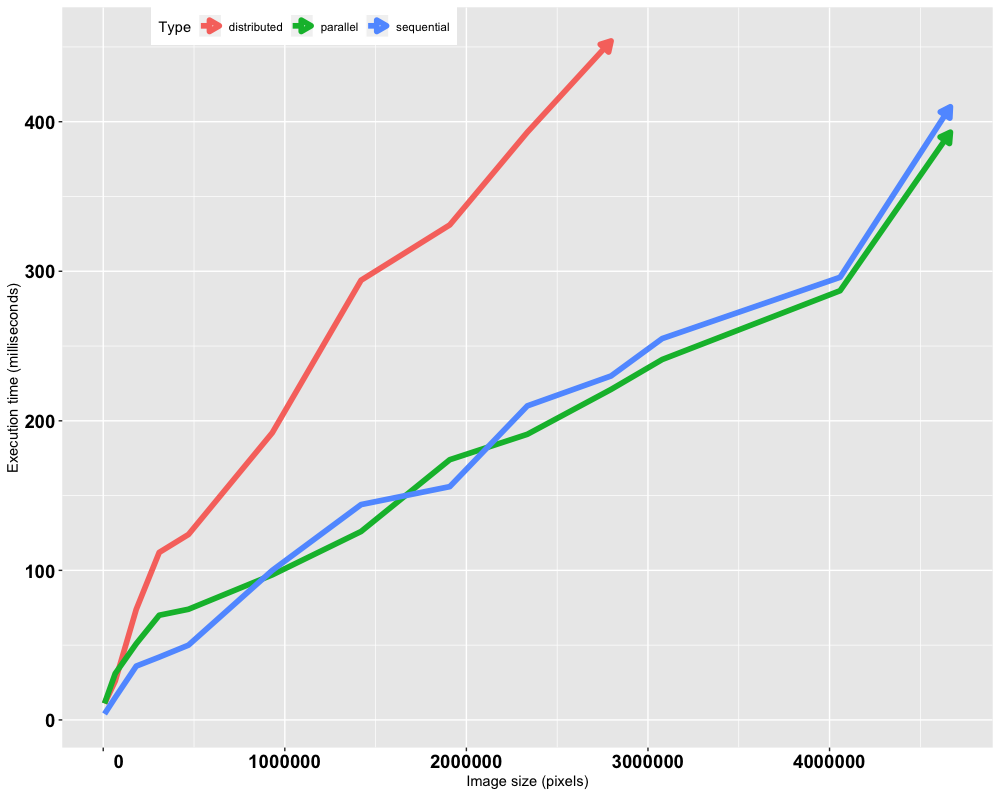
\includegraphics[width=\linewidth]{bigBefore.png}
  \caption{\textit{Execution time compared to image size}}
\end{figure}

\textit{Figure 2} shows results when for every execution and each image program was executed after first run (\textit{after image was proccesed, \textbf{program was not terminated } for new image})
\\
\setlength{\textfloatsep}{0pt}
\begin{figure}[h]
  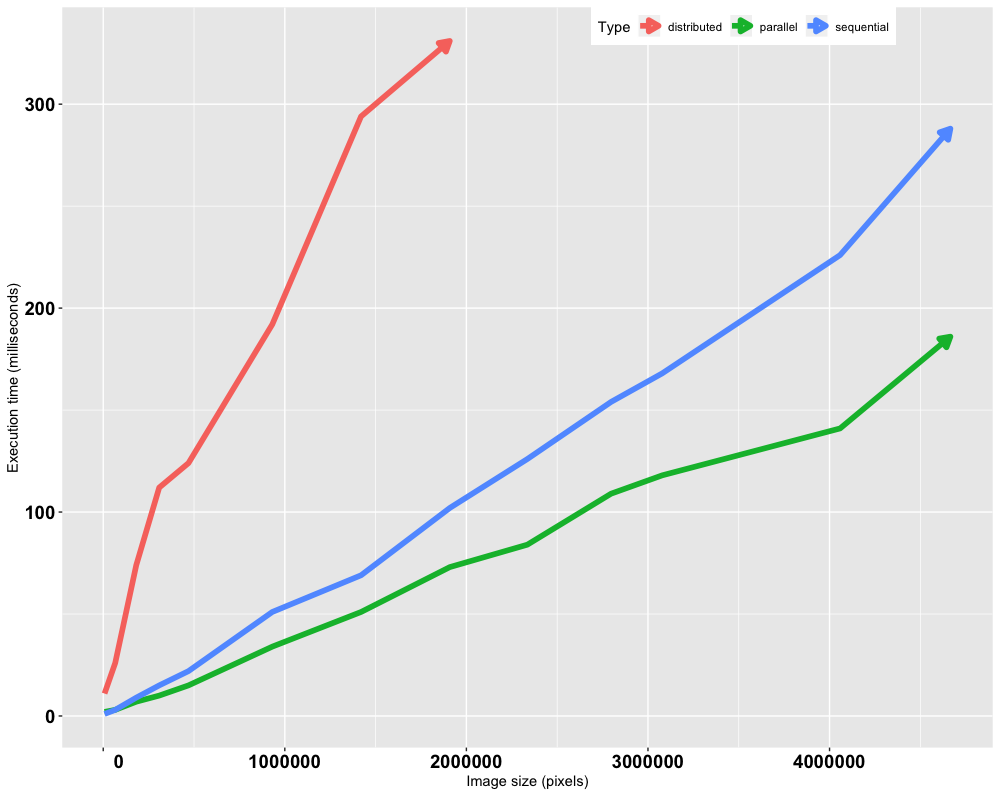
\includegraphics[width=\linewidth]{bigAfter.png}
  \caption{\textit{Execution time compared to image size}}
\end{figure}

\section{Conclusion}

Drawing a conclusion from \textit{Figure 1} and \textit{Figure 2 } we can state that Parallel implementation is far the best option in our case. It does take advantage of slicing the data and processing it independently, but does not allocate new memory. It runs much faster then sequential and distributed execution.

 Referencing to \textit{Figure 1}, we can realize that actual running up  the whole program takes time and also impacts first program execution of each implementation (\textit{Sequential, Parallel and Distributed}). 
 
 Chances are that Distributed implementation stumbles due to waste of memory and conversions of data types, which could be improved if we changed all three algorithms to work with contiguous arrays, instead matrices. This would lead to overall slower algorithms, but distributed would run faster, surely.
 
 \section{Repository}
Complete project repository including this report is available on my profile on Gitlab and Github: 
\\ 
\\
\textbf{Gitlab}: \textit{https://gitlab.com/elmirisz/Programiranje3}
\\
\textbf{Github}: \textit{https://github.com/elmirisz/Programiranje3}
\end{document}










